% -*- root: ../main.tex -*-

% Devono essere esposte le scelte progettuali operate nelle varie fasi di sviluppo dell'elaborato. In questa sezione devono essere documentati gli schemi di progetto relativamente all'architettura complessiva del sistema e alle sue componenti di rilievo che possano meritare un'analisi di dettaglio. Per le componenti software si può ricorrere ad esempio a diagrammi delle classi, di sequenza, stato, attività. Per le componenti hardware è possibile includere opportuni schemi in grado di descrivere l'architettura fisica adottata.

\chapter{Design Architetturale}

    \section{Architettura Generale}
    
    Abbiamo deciso di dividere il nostro sistema in due macro componenti: un applicativo server, che si occupi di gestire le richieste degli utenti, e un applicativo client, che si occupi di interrogare il server per richiedere informazioni. Le specifiche imposte dalla prova di esame in corso imponevano di usare determinate tecnologie per lo sviluppo di tali componenti, ma non imponevano altri vincoli. Abbiamo scelto noi di sviluppare i due componenti come progetti separati per aumentare l'indipendenza di un componente rispetto l'altro.
    
    \par Le funzioni da qui demandate all'applicativo \textbf{Server} sono:
    
    \begin{itemize}
    
        \item Richiesta di previsioni meteo da providers esterni: ci siamo registrati ai seguenti provider di previsioni meteo internazionali:
        
        \begin{itemize}
            
            \item Open Weather Map
            \item Troposphere
        
        \end{itemize}
        
        Quando il server viene interrogato per una previsione, la richiede a sua volta alle sorgenti di dati disponibili, che possono essere:
        
        \begin{itemize}
            \item Servizi esterni (sopra citati)
            \item Centraline degli utenti registrati
        \end{itemize}
        
        Non appena i risultati saranno ricevuti, sono immediatamente processati e forniti in output. Le unità di misura devono essere tutte uniformi e convertite all'occorrenza.
        
        \item Richiesta di autenticazione da parte dei client: date le credenziali degli utenti, il server si deve occupare di verificarne la presenza nella base dati degli utenti registrati nel sito. Dopo averne verificato l'autenticità e la validità, deve rilasciare un token di autenticazione da utilizzare nel caso in cui bisognasse richiedere delle risorse protette.
        
        \item Richiesta di feedbacks dei providers meteo: fornire un sistema di recensioni, le quali possono essere lasciate per ogni provider in base alla correttezza delle sue previsioni meteo. Successivamente calcolare la valutazione media di ogni servizio consultabile.
        
        \item Notifica di previsioni meteo a caselle di posta elettronica: configurando un account di posta elettronica per il proprio utente, il server deve poter inviare delle emails a chi ne fa richiesta per poter conoscere, all'inizio della propria giornata o nel momento che si ritiene più opportuno, le previsioni per la località preferita.
        
    \end{itemize}
    
    \par Le funzioni da qui demandate all'applicativo \textbf{Client} sono:
    
    \begin{itemize}
    
        \item Presentazione del progetto, degli autori e delle funzionalità messe a disposizione.
        
        \item Fornitura di un'interfaccia utente semplificata per la richiesta delle previsioni meteo all'applicativo Server:
        
        \begin{itemize}
            \item che renda comodo ed intuitivo la consultazione e la fruizione delle previsioni meteo dei vari providers
            
            \item che calcoli in automatico le statistiche relative alla distribuzione, alle differenze e similitudini dei risultati ottenuti dalle api
        \end{itemize}
        
        \item Gestione delle impostazioni e dei dati personali degli utenti: registrandosi al sito, ogni utente fornisce un insieme di dati e informazioni che devono essere mantenute, consultabili e modificabili agilmente. Le informazioni gestite comprendono anche la località preferita dell'utente, le centraline registrate e i feedbacks rilasciati.
        
        \item Gestione dei feedbacks rilasciati dagli utenti: deve rendere possibile creare delle recensioni per i providers e renderle consultabili da tutti gli utenti, assieme alla valutazione media del servizio stesso.
    
    \end{itemize}
    
    \par Oltre a questi componenti deve essere sviluppato anche il componente per simulare una centralina meteo amatoriale che possa ricevere le richieste del server per ottenere le previsioni meteo della zona in cui è situata. Per fare questo, abbiamo creato un nuovo progetto indipendente che assolva a questi compiti.

    \begin{figure}[H]
        \caption{Architettura Generale}
        \label{fig:General}
        \centering
        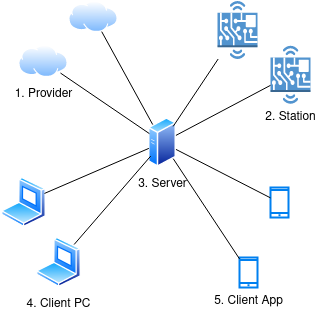
\includegraphics[width=0.5\textwidth]{DrawIo/General.png}
    \end{figure}
    
    \par Nel seguente schema vengono anche mostrati altri due componenti, chiamati Providers, che rappresentano i servizi esterni a cui ci affidiamo per ottenere dei dati meteo veritieri.
    
    \section{Scelte Tecnologiche Cruciali}
    
    Avendo l'esigenza di fornire all'utente i risultati delle previsioni meteo da lui richieste non appena essi fossero stati pronti, una scelta cruciale per il progetto è stata scegliere riuscire una tecnologia per mantenere un canale dati aperto tra il Client e il Server. Il protocollo HTTP non fornisce di per se un meccanismo tale per cui sia il Server ad inviare una richiesta di connessione al Client. Per questo motivo si è optato ad un approccio basato sulle Sockets. In particolare, abbiamo scelto la libreria \textit{Sockets.IO}, già vista a lezione.

    \section{Pattern Architetturali Utilizzati}
    
        
    
        \subsection{Client-Server}
        
            Nella figura 5.2 è illustrato come avviene un flusso di richieste di previsioni meteo dal Client al Server.
        
            \begin{figure}[H]
            
                \caption{Diagramma delle attività di una richiesta di previsioni dal Client al Server}
                
                \label{fig:Forecast Request Activity Diagram}
                
                \centering
                
                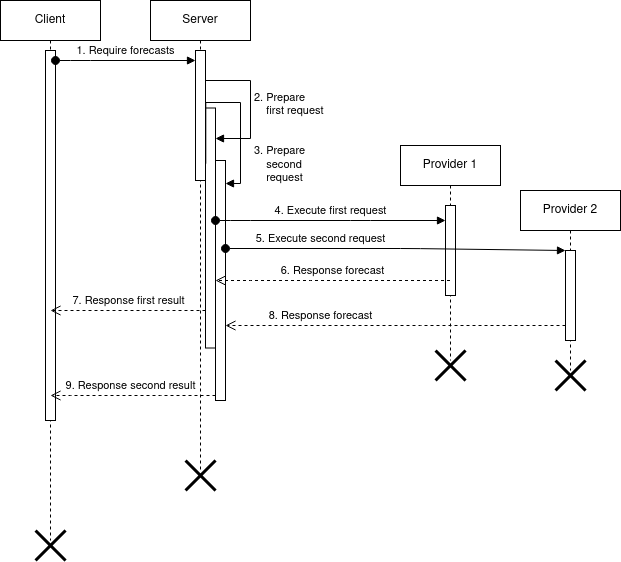
\includegraphics[width=0.75\textwidth]{DrawIo/forecast_request_activity_diagram.png}
                
            \end{figure}
            
            Procedendo in ordine numerico, al punto 1., il Client invia una richiesta al Server contenente il nome della località di cui vuole sapere le coordinate. Il Server nei punti 2. e 3. prepara la richiesta da inviare ai vari provider di previsioni meteo. Nello specifico vengono preparate solamente altre due richieste per altrettanti providers, ma in un caso reale potrebbero essercene molte di più. Da notare come in questo punto avvenga una divisione del flusso computazionale principale in due flussi separati ed indipendenti. Nei punti 4. e 5. tali flussi eseguono autonomamente le richieste delle previsioni al provider meteo esterno a loro assegnato. Ricevuta la risposta nei punti 6. e 7., la inoltrano al Client nei punti 7. e 8..